% -*- coding: utf-8 -*-

\chapter{自動行動計画問題 (Automated Planning Problem)}
%\chapter{古典的プランニング問題 (Classical Planning Problem)}
\label{ch:classical-planning}

本書の冒頭でグラフ探索アルゴリズムが人工知能のための技術として研究されていると説明した。
人工知能とはさまざまな定義で使われる言葉であるが、グラフ探索は自動推論や自動行動計画のために使うことができるために研究されている。
この章では人工知能の一分野である\define{自動行動計画問題}{automated planning problem}{じどうこうどうけいかくもんだい}について説明する \cite{ghallab:04}。
自動行動計画は初期状態から命題集合で表される目的を達成するための{\bf プラン}を発見する問題である。
自動行動計画のためのモデルは様々提案されている。
最も基本となるモデルは古典的プランニング問題である \cite{fikes:71}。
古典的プランニングは完全情報\footnote{正確には完全情報ではなく、アクションの決定のために必要な情報がすべて得られると仮定される。例えば問題に全く関係ない冗長な変数が含まれ、その情報がエージェントに与えられない場合は完全情報ではないが、アクションの決定のためには不要な情報であれば古典的プランニング問題で扱うことができる。}、決定的状態遷移を仮定とするモデルであり、状態空間問題に含まれる \cite{fikes:71}。
古典的プランニングによって様々な実問題を表すことができる。例えばロジスティック\cite{helmert2010scanalyzer,sousa2013toward}、セルアセンブリ\cite{asai2014fully}、遺伝子距離計算\cite{erdem2005genome}、ビデオゲーム\cite{lipovetzky2015a}など、様々な応用問題を含むモデルである。

\section{定義}
\label{sec:planning-definition}

古典的プランニング問題の最も基本となるSTRIPSモデル\cite{fikes:71}に従って定義する。

\ddef{
  STRIPS問題$P = (AP, A, s_0, Goal)$は命題変数の集合$AP$、アクションの集合$A$、初期状態$s_0 \subseteq AP$、ゴール条件$Goal \subseteq AP$からなる。
  アクション$a \in A$には適用条件$pre: A \rightarrow 2^{AP}$、追加効果$add: A \rightarrow 2^{AP}$、削除効果$del: A \rightarrow 2^{AP}$からなる。アクション$a$は適用条件$pre(a)$の命題を全て含む状態にのみ適用可能である。追加効果$add(a)$はアクション$a$を適用すると状態に追加される命題の集合であり、削除効果$del(a)$はアクション$a$を適用すると削除される命題の集合である。
  古典的プランニングの目的は与えられた初期状態$s_0$からはじめ、ゴール条件に含まれる命題がすべて含まれる状態に到達するまでのアクションの列を求めることである。
}

STRIPS問題は状態空間問題の一種である。状態空間は$2^{AP}$であり、アクション$a$を状態$s$に適用後の状態$s' = a(s)$は
\begin{equation}
	a(s) = (s \cup add(a)) \setminus del(a)
\end{equation}
である。
状態空間問題であるので、状態空間グラフを考えることができ、ヒューリスティック探索によって解くことができる問題である。

上の定義では集合の言葉で定義したが、人工知能の言葉、命題論理の言葉で説明することもできる。
STRIPSモデルは\define{命題論理}{propositional logic}{めいだいろんり}で書かれたモデルである。
\define{閉世界仮説}{closed-world assumption}{へいせかいかせつ}を仮定し、真であると示されていない命題は全て偽であるとする。
状態$s_0 = p_1 \land p_2 \land ...$は命題論理で書かれた世界の状態である。
アクションの適用条件はアクションを適用するために真であるべき命題である。
追加効果はアクションを適用した後に真になる命題、削除効果は偽になる命題である。
ゴール条件はゴール状態で真であるべき命題である。

このように古典的プランニングは論理エージェントと非常に密接な関係がある。
古典的プランニングに興味がある方は\cite{russelln03}を参照されたい。


% TODO: PDDLの文字フォントを\textttに
\section{プランニングドメイン記述言語: Planning Domain Definition Language}
\label{sec:pddl}

Planning Domain Definition Language (PDDL) \cite{aeronautiques1998pddl}はプランニング問題を記述されるために用いられる言語の一つである。PDDLはプランニング問題を\define{一階述語論理}{first-order predicate logic}{いっかいじゅつごろんり}で表現する。
PDDLはドメイン記述とインスタンス記述の2つに分けられ、Lispのような文法で書かれる。
図\ref{fig:pddl-domain}と図\ref{fig:pddl-instance}はブロックスワールド問題のドメイン記述とインスタンス記述である。
ここでドメインとインスタンスは計算理論などで定義される\define{問題}{problem}{もんだい}と\define{インスタンス}{instance}{インスタンス}に対応する。
ドメイン記述は問いの集合を定義し、インスタンスはその個例に対応する。
例えば「グリッド経路探索問題」はドメインであり、そのうちの特定の一つのマップがインスタンスに対応する。
ドメイン記述には\define{述語}{predicate}{じゅつご} (\texttt{predicates})と\define{アクションスキーム}{action scheme}{アクションスキーム} (\texttt{action})がある。
インスタンス記述には\define{オブジェクト}{object}{オブジェクト} (\texttt{objects})と初期状態(\texttt{init})、ゴール条件(\texttt{goal})がある。
これら以外にも例えばオブジェクトの型などを定義することができるが、簡単のためここではこれら基本の文法のみを紹介する。

PDDLに記述された一階述語論理は命題論理に変換できる。
まず、命題集合$AP$は述語に含まれる変数にオブジェクトを割り当てることによって得られる。
図の例だと例えば\texttt{(on A B), (on A C), (ontable D),...}などの命題が$AP$に含まれる。
アクション集合$A$はアクションスキームに含まれる変数にオブジェクトを割り当てることによって得られ、アクションの変数は\texttt{parameters}に定義される。
アクション$a$の適用条件$pre(a)$はアクションスキームの\texttt{precondition}にオブジェクトを割り当てることで得られる。\texttt{effect}のうち\texttt{not}のついていない命題は$add(a)$に対応し、\texttt{not}のついた命題は$del(a)$に対応する。
例えばアクション\texttt{(pickup A)}の適用条件は{\texttt{(clear A), (ontable A), (handempty)}}、追加効果は{\texttt{(holding A)}}、削除効果{\texttt{(ontable A), (clear A), (handempty)}}である。
初期状態$s_0$は\texttt{init}の命題集合である。この例では{\texttt{(CLEAR C) (CLEAR A) (CLEAR B) (CLEAR D) (ONTABLE C) (ONTABLE A)}}である。
ゴール条件$Goal$は\texttt{goal}の命題集合である。つまり、ゴール状態集合$T$は$Goal$を含む状態の集合である。

PDDLのミソは一階述語論理によってプランニング問題を記述する点である。
状態空間に含まれる命題を一つ一つ記述するのではなく、述語とオブジェクトの組み合わせによって複数の命題をコンパクトに記述することができる。
また、インスタンス記述を変えることで同じドメインの異なるインスタンスをモデルすることができる。
例えばブロックスワールドのドメイン記述はそのままに、インスタンス記述のオブジェクトや\texttt{init}などを変えることで違う問いにすることができる。

PDDLは状態空間問題だけでなくより広く様々な問題を扱うことができる \cite{aeronautiques1998pddl,fox2003pddl2}。
Fast DownwardはPDDLの文法の多くをサポートしているので試してみるには便利である。

\begin{figure}
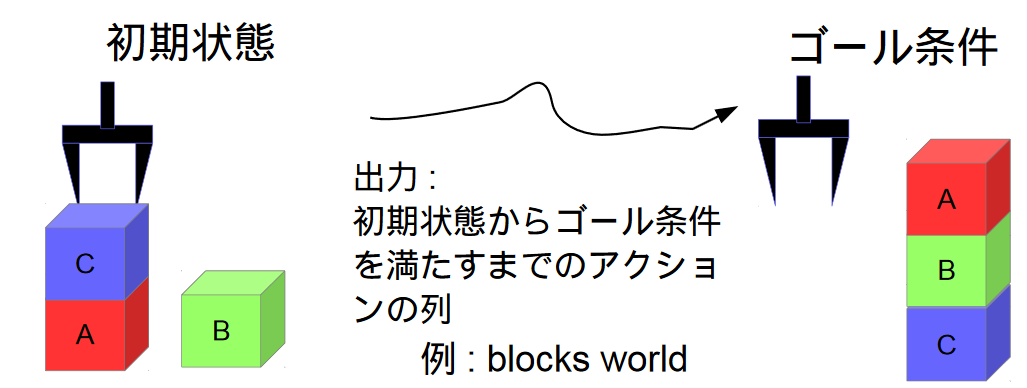
\includegraphics[width=0.8\linewidth]{./figures/blocks-image.png}
\caption{Blocks worldドメイン}
\label{fig:blocks-world}
\end{figure}

\begin{figure}
%\begin{adjustbox}{width=\textwidth,keepaspectratio}
\lstset{language=pddl,basicstyle=\ttfamily\footnotesize,breaklines=true}
\begin{lstlisting}
;;;;;;;;;;;;;;;;;;;;;;;;;;;;;;;;;;;;;;;;
;;; 4 Op-blocks world
;;;;;;;;;;;;;;;;;;;;;;;;;;;;;;;;;;;;;;;;
(define (domain BLOCKS)
  (:requirements :strips)
  (:predicates (on ?x ?y)
	       (ontable ?x)
	       (clear ?x)
	       (handempty)
	       (holding ?x)
	       )

  (:action pick-up
	     :parameters (?x)
	     :precondition (and (clear ?x) (ontable ?x) (handempty))
	     :effect
	     (and (not (ontable ?x))
		   (not (clear ?x))
		   (not (handempty))
		   (holding ?x)))

  (:action put-down
	     :parameters (?x)
	     :precondition (holding ?x)
	     :effect
	     (and (not (holding ?x))
		   (clear ?x)
		   (handempty)
		   (ontable ?x)))
  (:action stack
	     :parameters (?x ?y)
	     :precondition (and (holding ?x) (clear ?y))
	     :effect
	     (and (not (holding ?x))
		   (not (clear ?y))
		   (clear ?x)
		   (handempty)
		   (on ?x ?y)))
  (:action unstack
	     :parameters (?x ?y)
	     :precondition (and (on ?x ?y) (clear ?x) (handempty))
	     :effect
	     (and (holding ?x)
		   (clear ?y)
		   (not (clear ?x))
		   (not (handempty))
		   (not (on ?x ?y)))))
\end{lstlisting}
%\end{adjustbox}
\caption{blocks-worldのdomainファイル}
\label{fig:pddl-domain}
\end{figure}

\begin{figure}
%\begin{adjustbox}{width=\textwidth,keepaspectratio}
\lstset{language=pddl,basicstyle=\ttfamily\footnotesize,breaklines=true}
\begin{lstlisting}
(define (problem BLOCKS-3)
(:domain BLOCKS)
(:objects A B C)
(:INIT (CLEAR C) (CLEAR B) (ONTABLE C) (ONTABLE B)
 (ON C A) (HANDEMPTY))
(:goal (AND (ON A B) (ON B C)))
)

\end{lstlisting}
%\end{adjustbox}
\caption{blocks-worldのinstanceファイル}
\label{fig:pddl-instance}
\end{figure}

\section{古典的プランニング問題の例}
\label{sec:classical-planning-example}

プランニングは様々な問題解決に役立てることができる。
ここでは簡単にプランニングによってどのような問題がモデルできるかを紹介する。

\begin{enumerate}
\item エアポート (airport)
空港の地上の交通管理を行う問題である。
飛行機の離着陸の時間が与えられるのに対し、安全かつ飛行機の飛行時間を最小化する交通を求める問題である。

\item サテライト (sattellite)
人工衛星は与えられた現象を撮影し、地球にデータを送らなければならない。
このドメインはNASAの人工衛星の実際の応用から考案されたものである。

\item ローバー (rovers)
ローバーとは惑星探査ロボットのことである。
この問題は惑星探査ロボットのグループを使って惑星を探索する計画を作る問題である。
ロボットらは興味深い地形などの写真を取るなどの作業を実行する必要がある。
このドメインもNASAの応用をもとにしたものである。

\item パイプスワールド (pipesworld)
複数の原油の油田から複数の目的地にパイプを通して送りたい。
各目的地に定められた量を送るように調整することが目的である。
パイプのネットワークはグラフとしてモデルされており、また同時に原油を通せないパイプの組が存在する。

\item セルアセンブリ (cell assembly)
セルアセンブリは狭いセルの中で働き手が複雑な製品を作成する工場システムである。
大規模な製造ラインと比較して、
セルアセンブリは主に中程度の数(100個程度など)の製品を作るために使われる。
製品の開発や受注生産などに対応して、今生産しなければならない製品を手早く作成するためのセルの行動プランを考えることが問題の目的である。
\cite{asai2014fully}

\item ゲノムリアレンジメント (genome rearrangement)
ゲノムリアレンジメントは多重整列問題の一つである。
ゲノム間の編集距離とは類似性を測るための指標として使われ、生物の進化の歴史をたどるために使われる。編集距離はあるゲノムから操作を繰り返してもう一方のゲノムに変換するためのコストの総和として定義される。
プランニングモデルを用いることでより様々な操作を定義することができる。例えば遺伝子の位置に入れ替えなど、\ref{sec:msa}節で説明したように単純にグリッド経路探索に落とし込むことのできない複雑な操作を考えることができる。
\cite{erdem2005genome}

\item トラック (trucks)
ロジスティクスと呼ばれる問題の一種である。
トラックを運転してすべての荷物をそれぞれ定められた運び先に届ける問題である。
ただしトラックが運べる荷物の総量は有限であるため、それを考慮して経路を考えなければならない。加えて、届けるまでの期限が存在する荷物が存在する。

\end{enumerate}

これらの問題はすべて問題に特化した特別なアルゴリズムをそれぞれの問題に対して開発することもできる。多くの場合、特化アルゴリズムの方が汎用プランナーよりも高速である。プランナーの利点は問題に特化した実装をしなくてもPDDLを書くだけで問題を解くことが出来るという点にある。

\section{ヒューリスティック関数の自動生成}
\label{sec:automated-heuristic}

PDDLにはヒューリスティック関数は何を使えばよいかなどの情報は書かれていない。
よって、PDDLを入力とする状態空間問題を解く場合、エージェントはヒューリスティック関数を自動生成しなければならない。
PDDLからヒューリスティック関数を自動生成する手法はプランニング研究の最も重要な研究課題の一つである。

ヒューリスティックの生成方法の一つの指針としては\ref{sec:heuristic-example}節で言及した緩和問題によるヒューリスティックが分かりやすい。
すなわち、元の問題$P$よりも簡単な問題$P'$を生成し、$P$の状態$s$から$P'$の状態$s'$へのふさわしい関数を定義する。そして$h(s)$の値を$P'$における$s'$を初期状態とするゴールへの最適解にする。
このようにしてヒューリスティック関数は自動生成することができる。

各アルゴリズムの実装はfast-downward \footnote{\url{http://www.fast-downward.org}}を参照されたい。

\subsection{ゴールカウントヒューリスティック (Goal Count Heuristic)}

多くの問題ではゴールはいくつかの条件を満たした状態の集合として与えられる。
ゴールカウントヒューリスティックは満たしていないゴール条件の数をヒューリスティック値とする関数である。
例えばスライディングタイルのゴール条件は全てのタイルが所定の位置にあることである。
なので所定の位置にないタイルの数を$h$値とすることが出来る。

ゴールカウントヒューリスティックは許容的であるとは限らない。コスト1のアクションが2つのゴールを同時に満たすかもしれないからだ。1つのアクションで同時に満たせるゴールが1つ以下である場合、そしてその時のみ、許容的である。

\subsection{適用条件緩和 (Precondition Relaxation)}

\define{適用条件緩和}{precondition relaxation}{てきようじょうけんかんわ}はアクションの適用条件を無視し、すべてのアクションをすべての状態で適用できる緩和問題を解くヒューリスティックである。すべてのアクションが適用できるようになるので、グラフのエッジの数が増えることになる。このとき、すべてのゴール条件の命題は1ステップで満たすことができる。適用条件緩和はゴールカウントヒューリスティックに近いが、少しだけ適用条件緩和の方が正確である。なぜなら適用条件緩和の場合、1. 複数のゴールを同時に満たすアクションがある場合、そのアクションを1ステップで実行することができ、2. アクションを適用することによって一旦満たされた命題が削除されることがあるからである。適用条件緩和された問題は元の問題と比べて非常に簡単になっているが、まだまだ難しい。なので更に緩和し、一度満たされた命題が削除されないとすることが多い。
こうすると緩和問題は、追加効果$add(a)$の和集合がゴール条件を全て満たす$Goal \subseteq \bigcup_{a \in A'} add(s)$ような最小のアクション集合$A'$を求める問題になる。これはまさしく\define{集合被覆問題}{set cover}{しゅうごうひふくもんだい}である \cite{karp1972reducibility}。
集合被覆問題でもまだNP困難問題であるがシンプルな貪欲で$\log n$の近似アルゴリズムになる\cite{chvatal1979greedy}。
ただし近似アルゴリズムを使う場合、許容的なヒューリスティックではなくなってしまう。


\subsection{削除緩和 (Delete Relaxation)}

\define{削除緩和}{delete relaxation}{さくじょかんわ}はアクションの削除効果を無視する緩和問題を用いたヒューリスティックである \cite{hoffmann:01a}。この緩和問題では各アクション$a \in A$の代わりに$a^+$を用いる。$a^+$は$a^+$と同じ適用条件、追加効果を持っているが削除効果が空集合である ($del(a^+) = \emptyset$)。この緩和問題における最適解のコストをヒューリスティック関数$h^+$として用いる。
緩和問題では削除効果がないので状態に含まれる命題変数は単調増加していく。そのため元の問題よりも簡単になるが、これでもまだNP困難である \cite{bylander:94}。
そのため$h^+$を非許容的に見積もるヒューリスティック、例えばadditive heuristic \cite{bonet:01a}、FF heuristic \cite{hoffmann:01a}、pairwise max heuristic \cite{mirkis2007cost}、set-additive heuristic \cite{keyder2009trees}などがつかわれる。これらを用いた場合得られるヒューリスティックは非許容的になる。

$h^+$を許容的に見積もるヒューリスティックとしてはmax heuristic $h^{max}$がある \cite{bonet:01a}。$h^{max}$はゴール条件の各命題$t \in Goal$に対してその命題一つのみをゴール条件と更に緩和した問題 ($del(a^{max}) = \emptyset, Goal^{max} = t$)を解く。このコストを$c(t)$として、$h^{max}$はその最大値である ($h^{max} = \max_{t \in Goal} c(t)$)。
$h^{max}$は許容的であるが、非許容的なヒューリスティックよりも探索の効率が悪いこと多いことが実験的に示されている。
ちなみにadditive heuristicは最大値の代わりに$c(t)$の総和を取るものである。非許容的である代わりに$h^{max}$よりも性能が良いことが多い。

\subsection{最長経路 (Critical Path)}

\define{最長経路ヒューリスティック}{critical path heuristic} \cite{haslum:00}は命題の集合を全て満たすための最小コスト$c(X)$を$X$の大きさ$m$以下の部分集合$K \subseteq X$の最大値で近似する ($c^m(X) = \max_{X' \subseteq X, |X'| \leq m} c^m(X')$)というアイディアに基づいたヒューリスティックである。この近似は下界になるので許容的なヒューリスティックが得られる。max heuristicは最長経路ヒューリスティックのうち$m=1$の場合である ($h^{max} = h^1$)。$h^m \geq h^{m-1}$なので$m$が大きいほど正確な見積もりが出来るが、同時に計算コストが$m$に対して指数的に伸びるトレードオフがある。

元々GraphPlanと呼ばれる並行プランナーで使われたアイディアに基づいている \cite{blum:97}。

\subsection{抽象化 (Abstraction)}

\define{抽象化}{abstraction}{ちゅうしょうか}ヒューリスティックは状態$s$を抽象状態$\alpha(s)$への写像を用いたヒューリスティックである。
ヒューリスティック値$h^\alpha(s)$は抽象化された状態空間$S^\alpha = \{\alpha(s) | s \in S\}$でのゴールへの距離である。
抽象化は元の問題よりも簡単になるので許容的なヒューリスティックが得られる。
ヒューリスティックの性能は$\alpha$の選択による。
$\alpha$の選択方法としてはパターンデータベースヒューリスティック \cite{culberson1998pattern,edelkamp2001planning,holte:04,katz2008structural}、merge-and-shrink \cite{helmert2007flexible,helmert2014merge}などがある。

\subsection{ランドマーク (Landmark)}

プランニング問題の\define{ランドマーク}{landmark}{ランドマーク}とは、全ての解の中で一度でも真になることがある命題である \cite{porteous2001extraction}。
初期状態とゴール条件に含まれる命題はランドマークである。
ランドマークの直感的な理解としては、問題を解くために通過する必要がある中間目標地点である。

\define{ランドマークカウント}{landmark count}{ランドマークカウント}ヒューリスティックはこれから通過しなければならないランドマークの数をヒューリスティック値とする。
ランドマークを全て正しく発見する問題はPSPACE困難なので近似をする必要がある。
近似の方法によって非許容的なヒューリスティック (e.g. LAMA) \cite{richter2008landmarks}を得る手法と許容的なヒューリスティックを得る手法がある \cite{karpas2009cost}。

\define{ランドマークカット}{Landmark cut}{ランドマークカット}はランドマークカウントを一般化したヒューリスティックである \cite{helmert:09}。「全ての可能な解で真になる命題」はいくつかは発見できるが、十分な数を発見するのはかなり難しい。なのでランドマークカットはその代わりに「全ての可能な解で少なくとも一つが真になる命題の集合」を使う。このような命題の集合はjustification graphと呼ばれるランドマーク発見のためのグラフのカットに相当するため、ランドマークカットと呼ばれる。

% \section{プラン認識、ゴール認識}


\section{Python実装}

PDDLプランナーの多くはC, C++で実装されているが、Pythonで書かれたプランナーもある。
\define{pyperplan}{pyperplan}{パイパープラン}は著名なプランニングの研究者らがGPLv3で公開しているPythonで実装されたSTRIPSのプランナーである。
基本的な探索アルゴリズムや、ランドマーク、ランドマークカットなどのヒューリスティック関数、また本書では扱っていないが充足可能性問題 (SAT)のソルバーを利用したプランナーも実装されている。
pyperplanは\code{pip}からインストールできる。

\begin{python}
pip install pyperplan
\end{python}

例えばランドマークカットヒューリスティックでA*探索を行うプランナーを実行するには以下のようにする。

\begin{python}
pyperplan -H=lmcut --domain=domain.pddl --problem=problem.pddl
\end{python}

\section{まとめ}

ヒューリスティック探索はPDDLで記述された幅広い問題を自動行動計画問題として解くことができる。
ヒューリスティック関数は人間がデザインする必要はなく、PDDLから自動抽出した関数を利用して探索を効率化することができる。


\section{練習問題}
\begin{enumerate}
	\item グリッド経路探索問題をPDDLで記述し、それをpyperplanに入力して解いてみよう。
	
	\item いくつかのヒューリスティック関数を用いてグリッド経路探索問題を解いてみて、どのヒューリスティック関数が最も効果的かを調べてみよう。例えばランドマークカットとFFヒューリスティックではどちらが効率的だったか?
	
	\item (難問) ヒューリスティック探索は幅広い自動行動計画問題を解くことができる。では、それぞれ個別の問題を解くためのアルゴリズムを考える必要はあるのか?例えば巡回セールスパーソン問題はヒューリスティック探索以外だとどのような手法が使われているか?ヒューリスティック探索で解こうとすると、どのような問題があるのか?
\end{enumerate}

\section{関連文献}

自動行動計画を状態空間探索アルゴリズムで解くための手法はStefan Edelkamp and Stefan SchrodlのHeuristic Search Theory and Application \cite{edelkamp:2010:hst:1875144}にまとめられている。状態空間探索アルゴリズム以外にもSATやCSPなどの制約充足問題に変換して解く方法もある \cite{ernst1997automatic,do2001planning,sharon2015conflict}。

状態遷移が確率的である問題を\define{確率的プランニング}{probabilistic planning}{かくりつてきプランニング}と呼ぶ。確率的プランニングはマルコフ決定過程でモデルされることが多い。更に不完全情報である場合は\define{信念空間プランニング}{belief space planning}{しんねんくうかんプランニング}問題である。これらの問題は本文の範囲外とする。詳細は教科書を参照されたい\cite{russelln03}。

プランニングの問題定義やアルゴリズムの実装を見たい方はFast Downward \cite{helmert2006}をオススメする。
Fast DownwardはPDDLで表現された古典的プランニング問題を解くstate-of-the-artのプランナーである。
本書で紹介するアルゴリズムの多くがFast Downwardに組み込まれている。
